%%
%%
\begin{flushleft}
    {\fontsize{12}{0} \bf 實驗結果}
    \end{flushleft}
    %
    %
    \begin{abstract}
        \hspace{2em}
        \\ViT
        \\在ViT的模型訓練當中,觀察accurracy、loss曲線:
        \\1. 隨著learning rate增加,模型收斂的速度也隨之增快,若learning rate過低(如lr = 1*e-3),會有可能遇到模型收斂困難的問題。
        \\2. 模型訓練的準確度在epoch10~20的區間時就已經接近100\%,訓練集準確度接近100\%,但驗證集的準確率在收斂至約95\%時就不再收斂。
        \\3. 更改batch size參數,batch size提升時整體loss皆有下降的趨勢,準確率也有相對提升,不過隨著learning rate提升,改變batch size所造成的影響也隨之變小。
        \\
        \\在ViT的模型訓練當中,觀察confusion matrix與其指標:
        \\1. 對於同一個class,有時候Precision會低於Recall,有時Precision高於Recall,表示模型漏檢或是誤報的現象並不固定。
        \\2. 綜觀全部的class,表現最差class大多都落在open、short、spur,而open的表現最差,約落在90\%。
        \\
        \\加入GAN之後的變化:
        \\1. 對於整個訓練來說,隨著epoch增加的模型收斂速度有略為提升。
        \\2. 在較低learning rate當中的表現有得到不錯的提升,到了lr=1*e-5原本就很高的準確率也上升了1~2\%。    
    \end{abstract}
    %%
    \begin{figure}[!hbp] 
        \centering 
        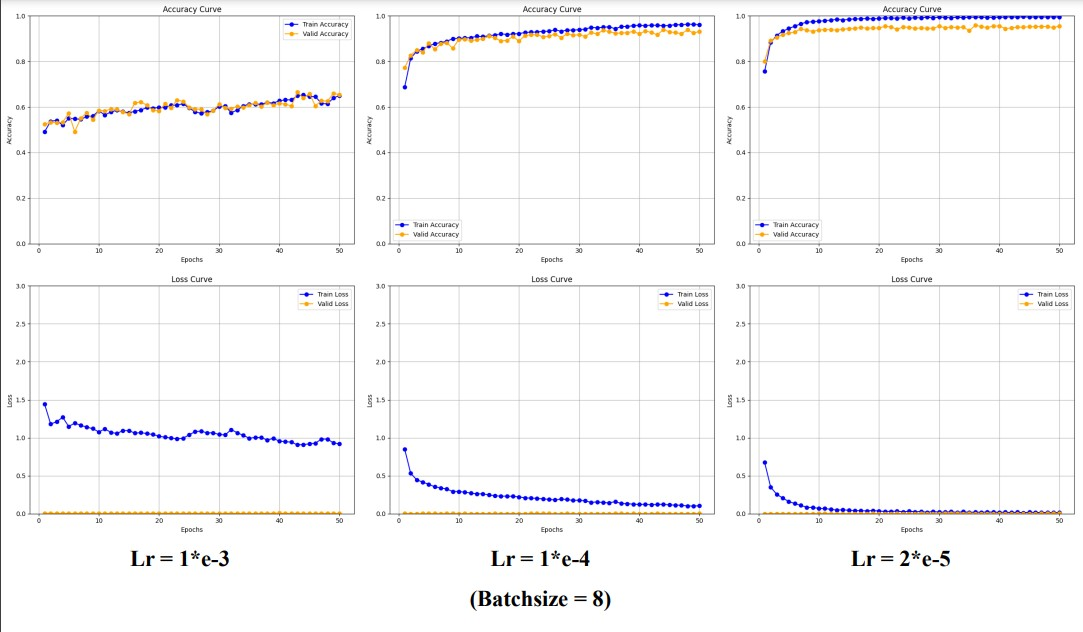
\includegraphics[width=0.85\linewidth, height=4cm]{img/ViT_b8.jpg} 
        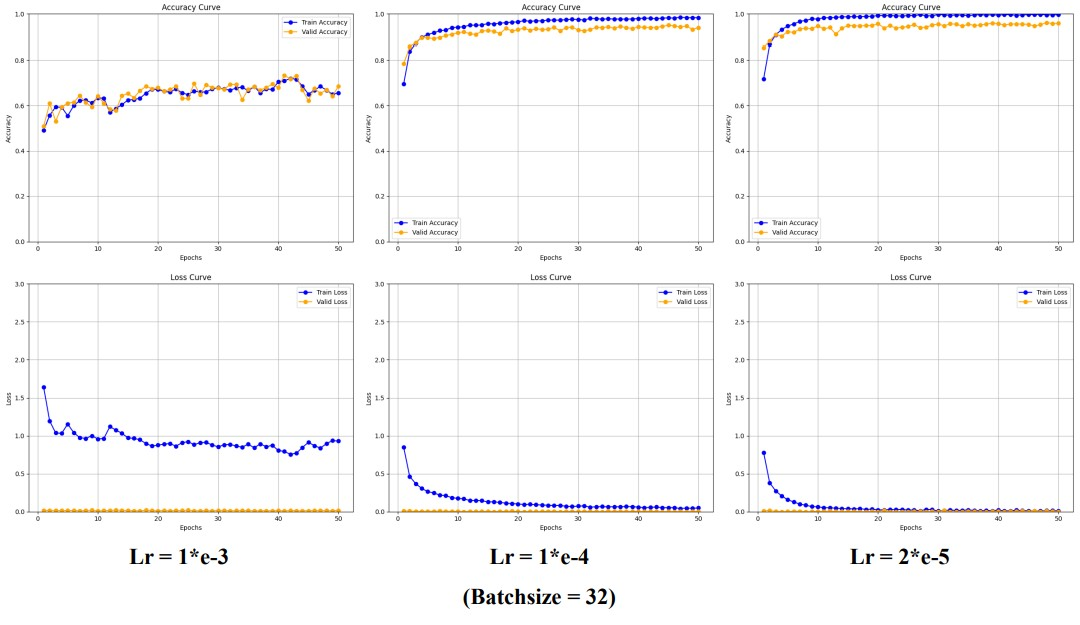
\includegraphics[width=0.85\linewidth, height=4cm]{img/ViT_b32.jpg}
        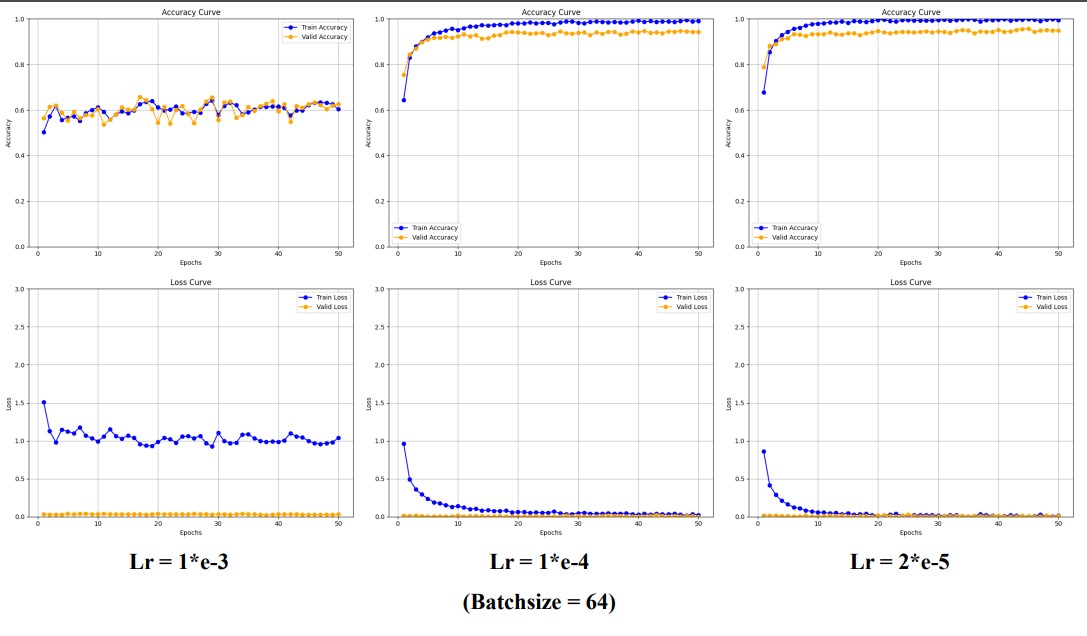
\includegraphics[width=0.85\linewidth, height=4cm]{img/ViT_b64.jpg}
        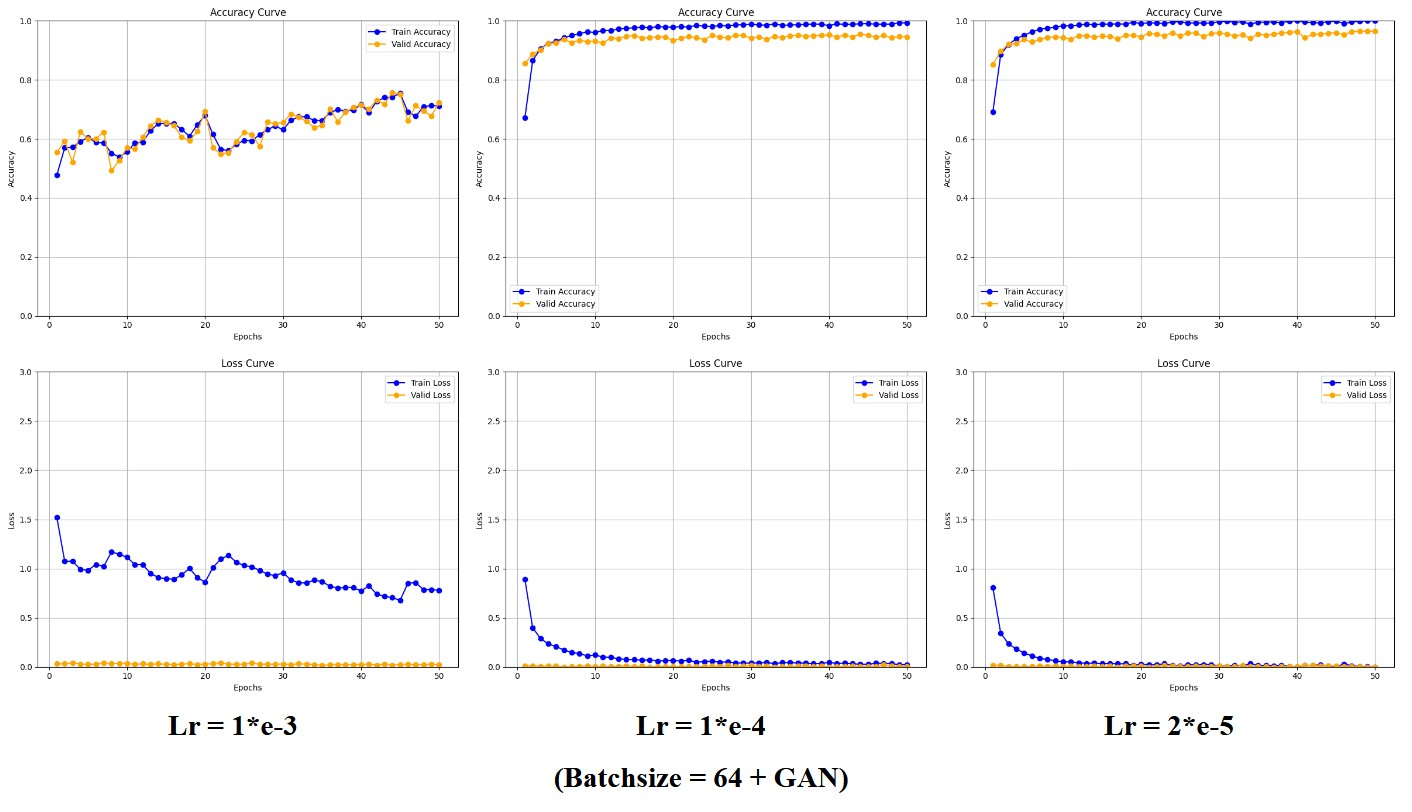
\includegraphics[width=0.85\linewidth, height=4cm]{img/ViT_b64_GAN.jpg}
        \caption{ViT訓練結果}
    \end{figure}
    %%
    \begin{abstract}
        \hspace{2em}
        \\ResNet
        \\在ResNet的模型訓練當中,觀察accurracy、loss曲線:
        \\1. ResNet在訓練中不論是有無使用GAN擴充的資料集,近乎都是呈現無法收斂的情況\ref{fig:ResNet_unconvergence_loss_curve},除了設定batch size為32,learning rate為1e-4或2e-5的情況有收斂完成\ref{fig:ResNet_convergence_loss_curve}。
        \\2. 在準確度上也對應了loss曲線的情況,因未成功收斂而導致準確度較差,在特定數據下才有準確率達到0.97的情況\ref{fig:ResNet_accuracy_curve}。
        \\3. 針對有使用GAN的資料集,在loss曲線有收斂完成的情況下,準確率較無使用GAN的資料集略低0.01左右。
        \\
        \\在ResNet的模型訓練當中,觀察confusion matrix與其指標:
        \\1. 對於同一個class,在loss曲線有收斂完成的情況下,precision與recall都達到0.96左右,而未完成收斂的情況則是precision明顯高於recall。
        \\2. 綜觀全部的class,最差的表現通常落在open、good,而以open的情況又較差\ref{fig:ResNet_confusion_matrix}。
    \end{abstract}
    %
    %
    \begin{abstract}
        \hspace{2em}
        \\SqueezeNet
        \\在SqueezeNet的模型訓練當中,觀察accurracy、loss曲線:
        \\1. SqueezeNet在不論是有無使用GAN進行擴充的資料集下,loss曲線幾乎都有收斂,除了在batch size為8與learning rate為1e-3,以本次實驗來說batch size極小learning rate極大的情況下,loss曲線完全沒有收斂,甚至是模型完全沒有學習到特徵。
        \\2. 而在learning rate為1e-3的情況下,多數的loss曲線會在epoch為10左右出現較大的起伏,進而影響到後面的模型收斂與最後的準確率。
        \\3. 準確度上因為多數情況下loss曲線都有收斂,所以準確度普遍落在0.96左右,在learning rate為1e-3,並且最後有收斂的情況下,準確率在0.69左右。
        \\4. 針對有使用GAN的資料集,在loss曲線有收斂完成的情況下,準確率與無使用GAN的資料集無明顯差異。 
        \\
        \\在SqueezeNet的模型訓練當中,觀察confusion matrix與其指標:
        \\1. 對於同一個class,在loss曲線有收斂完成的情況下,precision與recall都達到0.96左右,而未完成收斂的情況則是precision與recall數據持平,表示模型並沒有完整學習到特徵。
        \\2. 綜觀全部的class,最差的表現通常落在open、good,又以open的情況又較差。
    \end{abstract}
    %
    %    
    \begin{figure}[!t]
        \centering
        \includegraphics[width=0.45\textwidth]{../ResNet/runs/colorless_with_GAN/Fold2/train_e50_b64_lr0.001/train_valid_loss_curve.png}
        \caption{ResNet未收斂loss曲線}
        \label{fig:ResNet_unconvergence_loss_curve}
    \end{figure}
    %
    %
    \begin{figure}[!t]
        \centering
        \includegraphics[width=0.45\textwidth]{../ResNet/runs/colorless_with_GAN/Fold2/train_e50_b32_lr0.0001/train_valid_loss_curve.png}
        \caption{ResNet已收斂loss曲線}
        \label{fig:ResNet_convergence_loss_curve}
    \end{figure}
    %
    %
    \begin{figure}[!t]
        \centering
        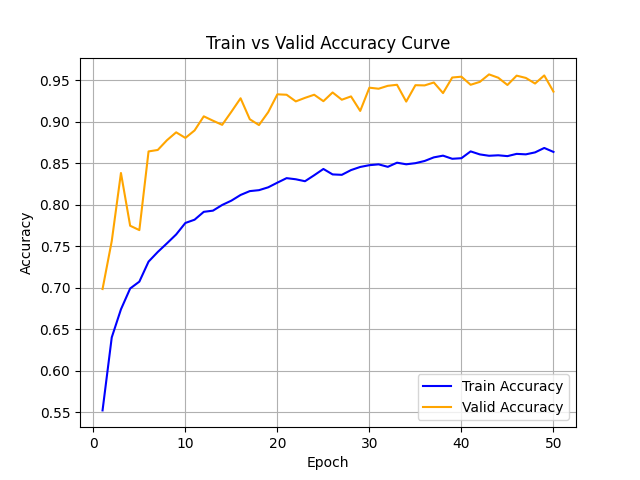
\includegraphics[width=0.45\textwidth]{../ResNet/runs/colorless_with_GAN/Fold2/train_e50_b32_lr0.0001/train_valid_accuracy_curve.png}
        \caption{ResNet Accuracy曲線}
        \label{fig:ResNet_accuracy_curve}
    \end{figure}
    %
    %
    \begin{figure}[!t]
        \centering
        \includegraphics[width=0.45\textwidth]{../ResNet/runs/colorless_with_GAN/Fold2/train_e50_b32_lr0.0001/confusion_matrix.png}
        \caption{ResNet Confusion Matrix}
        \label{fig:ResNet_confuson_matrix}
    \end{figure}
    %
    %
    
        